\subsubsection*{Grid Convergence Test}

The simulations of the flow in Vena Cava are conducted according to the parameters provided in \cite{craven_cfd}. The simulations of two flowrates are performed corresponding to the rest and exercise conditions. The density is $\rho=1817$, $\nu=3.21\times10^{-6}$ (rest) and $\nu=3.02\times10^{-6}$(exercise), and flowrate $Q= 0.5$ (l/min) and $3$ (l/min) into two iliac veins separately. The corresponding Reynolds numbers for rest and exercise conditions are 236 and 1505. The flow is considered to be laminar in the Vena Cava.
For boundary conditions, the parabolic velocity profile is prescribed at the inlet of two iliac veins. And the zero pressure condition is imposed at the outlet of the Vena Cava. 

For the mesh convergence test, 4 kinds of mesh sizes are used in the test. The mesh size and the total number of tetrahedral element for these 4 meshes are listed in the Table 1. The transverse cross-sections of all 4 meshes, which are located at 10 cm downstream of the after the merging location of two iliac veins, are shown in the Figure 1.

\begin{table}[h]
\caption {Mesh used in the convergence test.} \label{tab:meshsize}
\centering
\begin{tabular}{|c|c|c|}
\hline
Mesh & Number of element ($\times10^6$)& mesh size (mm) \\ \hline
1    & 0.87              & 2.0              \\ \hline
2    & 2.04              & 1.4            \\ \hline
3    & 4.70              & 1.0               \\ \hline
4    & 17.68             & 0.6            \\ \hline
5    & 37.94             & 0.45            \\ \hline
\end{tabular}
\end{table}

\begin{table}[h]
\centering
\caption {Value of maximum velocity, transverse velocity, Helicity and the correspoding convergence rates.} \label{tab:convergence}
\begin{tabular}{|c|c|c|c|c|c|c|}
\hline
     & \multicolumn{2}{c|}{maximum velocity} & \multicolumn{2}{c|}{transverse velocity} & \multicolumn{2}{c|}{Helicity} \\ \hline
Mesh & $\left |u\right |_{max} $    & p             & $\overline{\left |u\right |}_{tr}$          & p              &   $\overline{HI}$              & p           \\ \hline
1    & 0.25486               &               & 0.02380                 &                & 0.38067         &             \\ \hline
2    & 0.25846               &               & 0.02443                 &                & 0.41316         &             \\ \hline
3    & 0.25666               & 1.99533743    & 0.02474                 & 2.356          & 0.43313         & 1.63        \\ \hline
4    & 0.25409               & 0.70308244    & 0.02497                 & 0.311          & 0.44978         & 1.84        \\ \hline
5    &                       &               &                         &                &                 &             \\ \hline
\end{tabular}
\end{table}

\iffalse
\begin{table}[h]
\caption {} \label{tab:convergence}
\centering
\begin{tabular}{|c|c|c|c|}
\hline
Mesh & $u_{max}$ & Transverse velocity &  Helicity       \\ \hline
1    & 0.25486           & 0.02380        & 0.38067 \\ \hline
2    & 0.25846           & 0.02443        & 0.41316 \\ \hline
3    & 0.25666           & 0.02474        & 0.43313 \\ \hline
4    & 0.25409           & 0.02497        & 0.44978 \\ \hline
5    &                   &                &         \\ \hline
\end{tabular}
\end{table}
\fi

\subsubsection*{Comparison with Experimental Results}

\begin{figure*}
\begin{minipage}[c][9.5cm][c]{0.28\textwidth}
\centering
\vspace*{\fill}
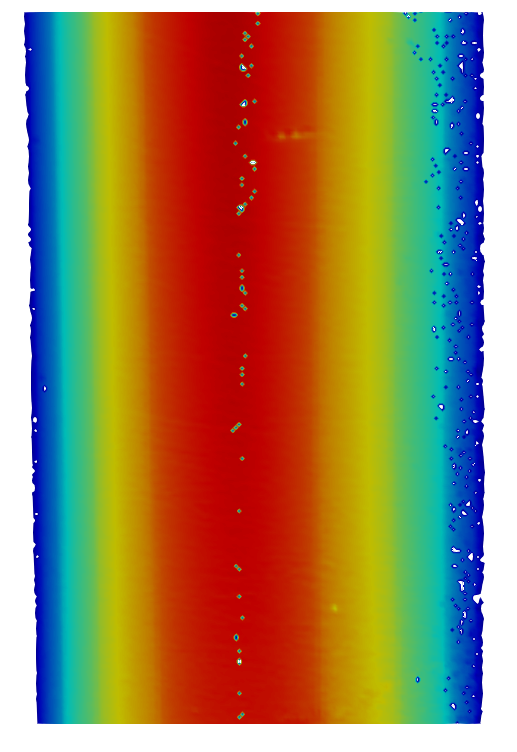
\includegraphics[height=4cm]{imgs/vena_cava/PIV_coronal_rest.png}
%\subcaption*{Step 1}
%\label{fig:process11}

%\addtocounter{subfigure}{1}
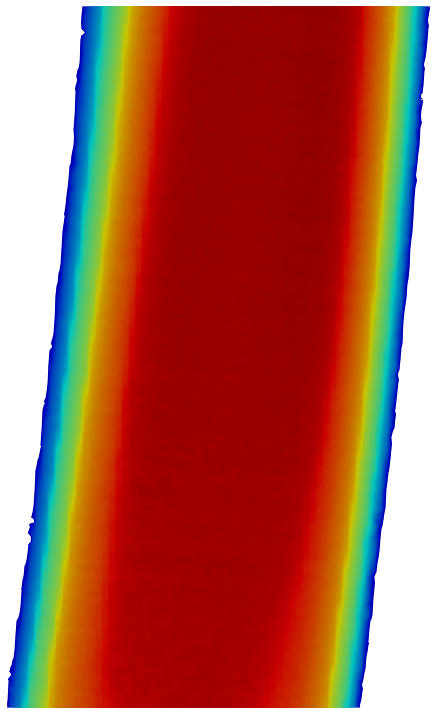
\includegraphics[height=5cm]{imgs/vena_cava/PIV_sagittal_rest.png}
PIV
%\subcaption*{PIV}
%\label{fig:process13}
\end{minipage}
\begin{minipage}[c][9.5cm][c]{0.28\textwidth}
\centering
\vspace*{\fill}
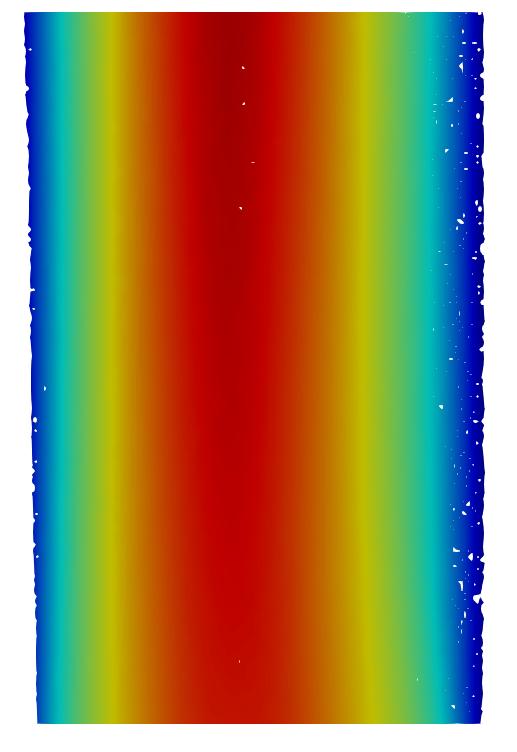
\includegraphics[height=4cm]{imgs/vena_cava/FEM_coronal_rest.png}
%\subcaption{Step 1}
%\label{fig:process11}

%\addtocounter{subfigure}{1}
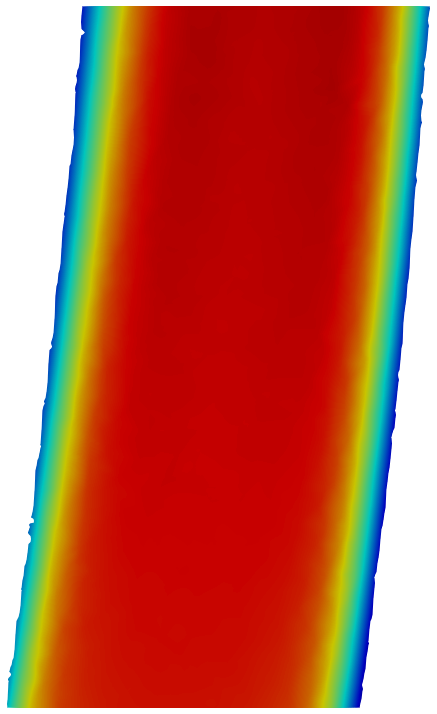
\includegraphics[height=5cm]{imgs/vena_cava/FEM_sagittal_rest.png}
FEM
%\subcaption*{FEM}
%\label{fig:process13}
\end{minipage}
\begin{minipage}[c][9.5cm][c]{0.28\textwidth}
\centering
\vspace*{\fill}
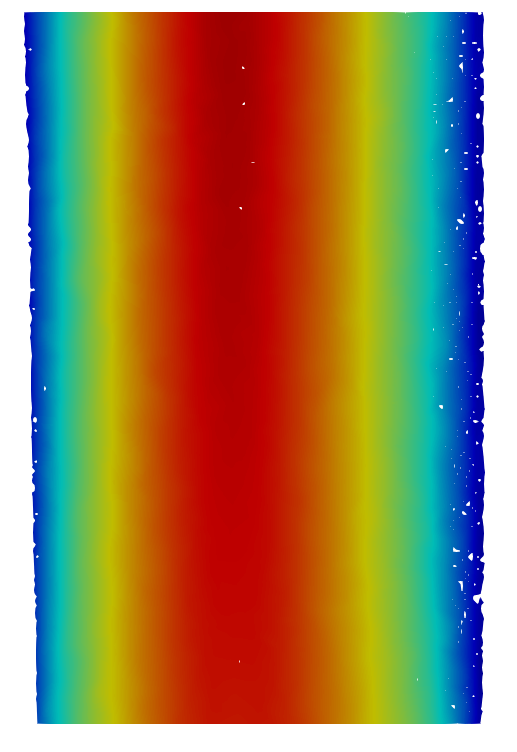
\includegraphics[height=4cm]{imgs/vena_cava/PFEM_coronal_rest.png}
%\subcaption{Step 1}
%\label{fig:process11}

%\addtocounter{subfigure}{1}
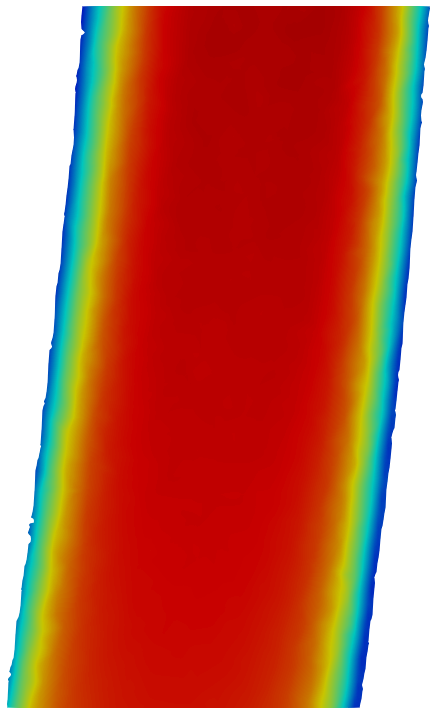
\includegraphics[height=5cm]{imgs/vena_cava/PFEM_sagittal_rest.png}
PFEM-2
%\subcaption*{PFEM-2}
%\label{fig:process13}
\end{minipage}
\begin{minipage}[c][9.5cm][t]{0.1\textwidth}
\vspace*{\fill}
\centering
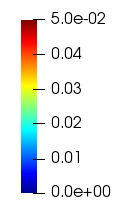
\includegraphics[height=3cm]{imgs/vena_cava/colormap_rest.png}
%\label{fig:process12}

\end{minipage}
\caption{The in-plane 2D velocity magnitude in coronal (top) and sagittal (bottom) planes of PIV, FEM and PFEM-2 results at resting condition}
\label{fig:process1}
\end{figure*}

\begin{table}[h]
\caption {Global relative error (\%) between CFD and PIV at resting condition} \label{tab:convergence}
\centering
\begin{tabular}{|c|c|c|}
\hline
       & Coronal & Sagittal \\ \hline
CFD from \cite{craven_cfd}  & 3.07    & 6.77     \\ \hline
FEM    & 4.83    & 6.62     \\ \hline
PFEM-2 & 4.79    & 6.65     \\ \hline
\end{tabular}
\end{table}

\begin{table}[h]
\caption {Global relative error (\%) between CFD and PIV at exercising condition} \label{tab:convergence}
\centering
\begin{tabular}{|c|c|c|}
\hline
       & Coronal & Sagittal \\ \hline
CFD from \cite{craven_cfd}  & 10.98	&5.56 \\ \hline
FEM    &      &    \\ \hline
PFEM-2 &     &       \\ \hline
\end{tabular}
\end{table}
